\section{Experiments}
\label{sec:experiments}


% \small

\normalsize

% \changnan{one paragraph deleted.}
% In this section, we firstly introduce our basic setup.
% Then we report our results on ALE, namely, 57 atari games. 
% To further investigate how CASA works, we study the effects of \textit{sg} operators, DR-Trace and path consistency.

% We also fix some game bugs, shown in Appendix \ref{app:bug_fix}.

\subsection{Basic Setup}
\label{sec:basic_setup}

We employ a Learner-Actor pipeline \citep{impala} for large-scale training.
% Our backbone is \textit{IMPALA,deep} \citep{impala}.
{\colorred Motivation and ablation experiments on PPO and R2D2 don't use LSTM, only experiments on CASA+DR-Trace use LSTM \citep{lstm}, which is for comparison with other algorithms.}
We use \textit{burn-in} \citep{r2d2} {\colorred when LSTM is used.}
All estimated values share the same backbone, which is followed by two fully connected layers for each individual head.
% We store recurrent states during inference and make it the initial hidden state of \textit{burn-in} phase.
% We train each sample twice.
% We replay each data point twice, by a smooth \textit{burn-in} shift.
% For any trajectory, we break up the trajectory into segments by an offset $\lfloor$\textit{burn-in} / 2$\rfloor$, where each data point is trained exactly twice.
We use no intrinsic reward and no entropy regularization in any experiment.
We find that using life information can greatly increase the performance of some games. 
However, to be general, we will not end the episode if life is lost.
All hyperparameters are in Appendix \ref{app:hyperparameters}.

{\colorred For brevity, we denote $\nabla L_V = \mathbb{E}_\pi [(V^\pi - V_\theta)\nabla V_\theta]$, $\nabla L_Q = \mathbb{E}_\pi [(Q^\pi - Q_\theta)\nabla Q_\theta]$ and $\nabla \mathcal{J} = \mathbb{E}_\pi [(Q^\pi - V_\theta)\nabla \log \pi_\theta]$, where expectation is batch-wise average in our implementation. 
When we write $<a, b>$ with $a, b \in \{\nabla L_V, \nabla L_Q, \nabla \mathcal{J}\}$, we firstly calculate batch-wise averaged gradient of $a$ and $b$, then we calculate the angle in-between. 
When we write $\cos<\nabla Q, \nabla \log \pi>$ or $\chi$, we mean $\mathbb{E}_\pi [\cos <\nabla_\theta Q_\theta, \nabla_\theta \log \pi_\theta>]$, which firstly calculates element-wise cosines and then takes batch-wise average.
To avoid numerical problem, we calculate $\frac{x\cdot y}{||x||\cdot||y||}$ by $\frac{x\cdot y}{\max(||x||, 10^{-8})\cdot \max(||y||, 10^{-8})}$.
}

\subsection{Application of CASA on Representative Algorithms}
\label{sec:on_ppo_and_r2d2}

\begin{table}[ht!]
    \centering
    \scalebox{0.86}{
    \begin{math}
        \begin{array}{c|ccc|ccc}
    \toprule
    & \text{PPO} &  & \text{PPO+CASA} & \text{R2D2} & & \text{R2D2+CASA} \\
    \midrule
    & & \multirow{4}{*}{$\Rightarrow$} & (V, A) = (V_\theta, A_\theta) & & \multirow{4}{*}{$\Rightarrow$} & (V, A) = (V_\theta, A_\theta) \\
    \text{Func.} & (V, logit) = (V_\theta, logit_\theta) & & \pi = \text{softmax}(A/\tau) & (V, A) = (V_\theta, A_\theta) & & \pi = \text{softmax}(A/\tau) \\
    \text{Approx.} & \pi = \text{softmax}(logit)& & \Bar{A} = A - sg(\pi) \cdot A & Q = A + V & & \Bar{A} = A - sg(\pi) \cdot A \\
    & & & Q = \Bar{A} + sg(V) & & & Q = \Bar{A} + sg(V) \\
    \midrule
    \text{Gradient} & 0.5 \nabla L_V + \nabla \mathcal{J} & \Rightarrow & 0.5 \nabla L_V + \nabla L_Q + \nabla \mathcal{J}  & \nabla L_Q & \Rightarrow & 0.5 \nabla L_V + \nabla L_Q + \nabla \mathcal{J} \\
    \bottomrule 
    \end{array}
    \end{math}
    }
    \caption{Examples of applying CASA on policy-based methods (PPO) and value-based methods (R2D2).}
    \label{tab:on_ppo_and_r2d2}
    \vskip -0.1in
\end{table}

CASA is applicable to existing algorithms. 
We take PPO and R2D2 for demonstration. 
The application of CASA on PPO is straightforward. 
Applying CASA on R2D2 is impossible as either $\epsilon$-greedy policy or $\arg\max Q$ policy breaks the gradient. 
This problem is the same as calculating the gradients of policy improvement for value-based methods.
We use a surrogate policy $\pi_{surrogate} = \text{softmax}(A / \tau)$, which is discussed in Appendix \ref{app:mtv}. 
Table \ref{tab:on_ppo_and_r2d2} summarizes adjustments of function approximations and training gradients. 

Since PPO+CASA and R2D2+CASA have the same function approximation, recalling the fact that value-based methods improve the policy when a more accurate evaluation is achieved and policy-based methods improve the policy for every step, we can balance the two flexibly with $\chi=1$ by $\alpha_1, \alpha_2, \alpha_3$ in \eqref{eq:grad_all}.

In Figure \ref{fig:mtv}, algorithms with CASA show much higher $\cos(\beta)$ and $\chi$. 
PPO+CASA does more exploration than the original PPO, as the entropy of $\pi$ doesn't easily drop to zero. 
R2D2+CASA tends to distinct the state-action values, where we use the entropy of $Q$ to measure how greedy the current state-action values are. % here we should show what is the entropy of Q
% We also include more angles that are interesting in Appendix \ref{app:mtv}.

\subsection{Behavior of Gradients on different structures}
\label{sec:ablation}

\begin{table}[ht!]
\centering
\begin{minipage}[b]{0.4\textwidth}
\scalebox{0.88}{
\begin{math}
\begin{array}{c|c}
\toprule
\text{PPO+CASA} & Q = A_\theta - sg(\pi_\theta) \cdot A_\theta + sg(V_\theta) \\
\midrule
\text{type 1} & Q = A_\theta - \pi_\theta \cdot A_\theta + sg(V_\theta) \\
\hline
\text{type 2} & Q = A_\theta - sg(\pi_\theta) \cdot A_\theta + V_\theta  \\
\hline
\text{type 3} &  Q = A_\theta + sg(V_\theta)  \\ 
\hline
\text{type 4} & Q = A_\theta + V_\theta  \\ 
\hline
\text{type 5} & Q = Q_\theta  \\
\bottomrule
\end{array}
\end{math}
}
\end{minipage}\hfill
\begin{minipage}[c]{0.56\textwidth}
\setlength{\abovecaptionskip}{0pt}%
\caption{\small Behavior of gradient on different types. Type 1$\&$2 are CASA-like structures, where type 1 removes $sg$ of $\pi$ and type 2 removes $sg$ of $V_\theta$. Type 3$\&$4 are dueling-like structures, where type 3 adds $sg$ to $V$ for dueling-Q and type 4 is dueling-Q. Type 5 uses a new head to estimate $Q_\theta$ separately, which can be considered as an auxiliary task to estimate $Q^\pi$. }
\label{tab:ablation_parameters}
\end{minipage}
\end{table}

Though we show that CASA satisfies $\nabla Q \propto \nabla \log \pi$, {\colorred which means $\chi = 1$}, it's unknown if the structure of CASA is unique. 
As $Q = A - \mathbb{E}_\pi[A] + sg(V)$ is a direct refinement of dueling-DQN, we try several different structures of PPO+CASA. 
All settings of estimating state-action values are shown in Table \ref{tab:ablation_parameters}. 
We always use $0.5 \cdot \nabla L_V + \nabla L_Q + \nabla \mathcal{J}$ as the training gradient. 
We present Breakout and Qbert in Figure \ref{fig:ablation}.
% \haosen{Noted, we may choose other games with higher performance.} 
% {\colorred We observe $\chi$ and cosines of angles between $\nabla L_V$, $\nabla L_Q$ and $\nabla \mathcal{J}$.}


% \begin{table}[ht!]
% \centering
% \scalebox{0.90}{
% \begin{math}
%     \begin{array}{c|c}
% \toprule
% \text{PPO+CASA} & Q = A_\theta - sg(\pi_\theta) \cdot A_\theta + sg(V_\theta) \\
% \midrule
% \text{type 1} & Q = A_\theta - \pi_\theta \cdot A_\theta + sg(V_\theta) \\
% \hline
% \text{type 2} & Q = A_\theta - sg(\pi_\theta) \cdot A_\theta + V_\theta  \\
% \hline
% \text{type 3} &  Q = A_\theta + sg(V_\theta)  \\ 
% \hline
% \text{type 4} & Q = A_\theta + V_\theta  \\ 
% \hline
% \text{type 5} & Q = Q_\theta  \\
% \bottomrule
% \end{array}
% \end{math}
% }
% \caption{Behavior gradient types. Type 1 and type 2 are CASA-like structures, where type 1 removes $sg$ of $\pi$ and type 2 removes $sg$ of $V_\theta$. Type 3 and type 4 are dueling-like structures, where type 3 adds $sg$ to $V$ for dueling-Q and type 4 is dueling-Q. Type 5 uses a new head to estimate $Q_\theta$ separately, which can be considered as an auxiliary task to estimate $Q^\pi$. }
% \label{tab:ablation_parameters}
% \end{table}


\begin{figure*}[t!]
\centering
% \subfigure[FIGTOPCAP][breakout]{
% % \begin{minipage}{.33\linewidth}
% \includesvg[width=0.22\linewidth,inkscapelatex=false]{body/ablation/Breakout_nips1_ab.svg}
% }
% \subfigure[FIGTOPCAP][chopper\_command]{
% \includesvg[width=0.22\linewidth,inkscapelatex=false]{body/ablation/Chopper_Command_nips1_ab.svg}
% }
% \subfigure[FIGTOPCAP][krull]{
% \includesvg[width=0.22\linewidth,inkscapelatex=false]{body/ablation/Krull_nips1_ab.svg}
% }
% \subfigure{
%     \includegraphics[width=0.20\linewidth]{body/ablation/label_nips1_ab.pdf}
%     % \begin{minipage}[t]{7cm}
%     % \centering
%     % \raisebox{0.3\height}{\includegraphics[width=0.25\columnwidth]{nips1/ablation/label_nips1_ab.pdf}}
%     % \end{minipage}
% }
% \includegraphics[width=0.9\linewidth,bb= 0 0 1400 375]{body/ablation/ablation.pdf}
\includegraphics[width=1.0\linewidth]{body/intro_fig/new_ab_Breakout.pdf}
\includegraphics[width=1.0\linewidth]{body/intro_fig/new_ab_Qbert.pdf}
\caption{The ablation results evaluated on Breakout (top row) and Qbert (bottom row). From left to right is the \emph{return} curve, $\chi$, $\cos(\beta)$, \emph{scatter plot} of $(\chi, \cos(\beta))$ and \emph{box plot} of $(\chi, \cos(\beta))$. Each scatter point is one batch sampled from every consecutive 100 batches. Each box is the interquartile range of scatter points.
}
\label{fig:ablation}
 % \vskip -0.1in
\end{figure*}

For the sake of clarity, we group PPO+CASA and type 3 as $sg\text{-}V$ group, type 2 and type 4 as $no\text{-}sg\text{-}V$ group. 
{\colorred The $sg\text{-}V$ group has higher $\chi$ and higher $\cos(\beta)$, which is closer to the compatible condition and the consistency between two GPI steps,} 
% The $no\text{-}sg\text{-}V$ group has higher {\colorred $\cos<\nabla L_Q, \nabla L_V>$}, which is simple to explain as the gradient of $Q$ also includes the gradient of $V$. 
% However, this seems to be hard for distinguishing state-action values, as
and $no\text{-}sg\text{-}V$ group is always worst than its contrast in $sg\text{-}V$ group. 

{\colorred PPO+CASA has $\chi=1$ and the highest $\cos(\beta)$. }
Type 1 has less returns than PPO+CASA. 
Hence, when applying a CASA-like structure, stopping the gradient of $\pi$ is always preferred. 

{\colorred Type 5 uses an individual head to estimate $Q^\pi$, which performs the worst. 
Hence, a well-designed CASA-like or dueling-like structure is always preferred. }

{\colorred By scatter plot and box plot in Figure \ref{fig:ablation}, $\chi$ and $\cos(\beta)$ are positive correlated depending on different structures.
This phenomenon answers part of the last question of Section \ref{sec:motivation}: for these specific designed structures, $\chi$ and $\cos(\beta)$ show positive correlation. }

% Type 5 only adds an auxiliary task of estimating $Q^\pi$ by $Q_\theta$ via $\nabla L_Q$, but surprisingly fails learning in all games. 
% It reflects the fact that even the gradient from an explainable auxiliary target function can cause great failure. 
% It's surprising to see that cosines of all four angles of type 5 are very close to zero. 
% One can explain this as all gradients are pulling each other, but this is far from satisfactory. 
% This phenomenon shows a potential condition to decide what a good auxiliary task may be. 

% \changnan{old ablation table deleted}
% \label{sec:ablation}
% \begin{table*}[t]
%     \centering
%         \caption{Ablation Settings. The baseline of these ablation changes is \textbf{original CASA}. Except for the changes listed in the table, there is no other change of CASA in each ablation case.}
%     \vspace{0.2cm}
%     \resizebox{.78\textwidth}{!}{
%     \begin{tabular}{cccc}
%     \toprule
%     \textbf{Name} & \textbf{Origin} & & \textbf{Change(s)}  \\
%     \midrule
%         CASA 
%         & N/A 
%         & & N/A \\
%     \midrule
%         \textit{no\_stop\_$\pi$} 
%         & $\Bar{A} = A - \mathbb{E}_\pi[A] = A - sg(\pi) \cdot A$ 
%         & $\Rightarrow$ & $\Bar{A} = A - \pi \cdot A$ \\
%     \midrule
%         \textit{no\_stop\_v} 
%         & $Q = \Bar{A} + sg(V) $ 
%         & $\Rightarrow$ & $ Q = \Bar{A} + V$ \\
%     \midrule
%         \textit{no\_drtrace} 
%         & $V_\theta$ is estimated by DR-Trace
%         & $\Rightarrow$ & $V_\theta$ is estimated by V-Trace \\
%         & $Q_\theta$ is estimated by DR-Trace
%         & $\Rightarrow$ &  $Q_\theta$ is estimated by ReTrace \\
%     \midrule
%         \textit{random\_scaling}
%         & $Q$-loss Scaling $\alpha_2 = 10.0$ 
%         & $\Rightarrow$ & $ \alpha_2 \sim Uniform([0.0, 20.0])$ \\
%         & $\pi$-loss Scaling $\alpha_3 = 10.0$ 
%         & $\Rightarrow$ & $ \alpha_3 \sim Uniform([0.0, 20.0])$ \\
%     \bottomrule
%     \end{tabular}
%     }

%     \label{tab:ablation_parameters}
% \end{table*}

% \changnan{old ablation setting paragraph deleted}
% We check the following aspects of CASA.
% \textbf{(i)} \textit{stop gradient} of $\pi$ in $\Bar{A} = A - \mathbb{E}_\pi [A] = A - sg(\pi) \cdot A$, which gives the path consistency. 
% The ablation study removes $sg$ operator, so the path consistency cannot hold.
% \textbf{(ii)} \textit{stop gradient} of $V$ in $Q = \Bar{A} + sg(V)$, which is crucial in the convergence proof of Theorem \ref{thm:dr}.
% The ablation study removes $sg$, so the convergence property of DR-Trace cannot be guaranteed.
% \textbf{(iii)} DR-Trace, which is to reduce the variance of the policy evaluation maximally.
% The ablation study uses V-Trace to estimate state value and ReTrace to estimate state-action value instead of DR-Trace, which aims to check the efficiency of DR-Trace.
% \textbf{(iv)} The path consistency property between the policy evaluation and the policy improvement.
% Since the gradient directions of $Q$-loss and $\pi$-loss are identical, it should be less influenced by the scale of the step-size, which meets the motivation in Figure \ref{fig:gpi}.
% The ablation study samples the coefficients of $Q$-loss and $\pi$-loss for every sample of every batch.
% If the path consistency property holds, it should perform similar to the original CASA.
% All ablation settings are listed in Table \ref{tab:ablation_parameters}.

% \changnan{old ablation figures deleted.}
% \begin{figure*}[h]
% \centering
% % \subfigure[FIGTOPCAP][breakout]{
% % % \begin{minipage}{.33\linewidth}
% % \includesvg[width=0.22\linewidth,inkscapelatex=false]{body/ablation/Breakout_nips1_ab.svg}
% % }
% % \subfigure[FIGTOPCAP][chopper\_command]{
% % \includesvg[width=0.22\linewidth,inkscapelatex=false]{body/ablation/Chopper_Command_nips1_ab.svg}
% % }
% % \subfigure[FIGTOPCAP][krull]{
% % \includesvg[width=0.22\linewidth,inkscapelatex=false]{body/ablation/Krull_nips1_ab.svg}
% % }
% % \subfigure{
% %     \includegraphics[width=0.20\linewidth]{body/ablation/label_nips1_ab.pdf}
% %     % \begin{minipage}[t]{7cm}
% %     % \centering
% %     % \raisebox{0.3\height}{\includegraphics[width=0.25\columnwidth]{nips1/ablation/label_nips1_ab.pdf}}
% %     % \end{minipage}
% % }

% \includegraphics[width=0.22\linewidth]{body/r2d2_results/Break.pdf}
% 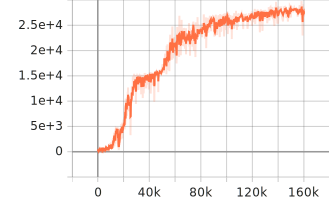
\includegraphics[width=0.22\linewidth]{body/r2d2_results/Qbert.pdf}
% 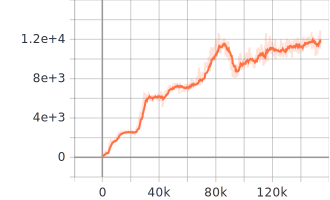
\includegraphics[width=0.22\linewidth]{body/r2d2_results/Seaquest.pdf}
% \caption{Evaluation Return Curves.(only for test) }
% % \vskip -0.2in
% \label{fig:ablation1}
% \end{figure*}

% \changnan{ablation game paragraph deleted}
% We do ablation study on three different games, Breakout, ChopperCommand and Krull.
% We choose Breakout because most algorithms can achieve a better result on it with a large training scale.
% But it's not easy to get an extreme high score on it. 
% So it's a good benchmark to verify the sample efficiency.
% We choose ChopperCommand and Krull, because we find there exists a breakthrough moment for each game.
% Some algorithms can make a breakthrough, while some cannot.
% We do not choose any hard-to-explore games for ablation study, such as Pitfall, MontezumaRevenge.
% This is because CASA is not designed to solve these problems and have not approached the average human performance on these games.
% It's not convincing to do ablation study when the baseline performs poor on these games.

% \changnan{ablation analysis paragraph deleted}
% Our ablation results are shown in Figure \ref{fig:ablation}.
% It's obvious that \textit{no\_stop\_$\pi$} and \textit{no\_stop\_v} perform the worst among others.
% They show a lower sample efficiency on Breakout and have not made a breakthrough on ChopperCommand and Krull.
% This phenomenon proves the two $sg$ operators defined in the definition of CASA \eqref{eq:casa} are necessary.
% One is for the path consistency property and the other is for the convergence property of DR-Trace.
% As for \textit{random\_scaling}, though it shows a lower sample efficiency on ChopperCommand and a higher sample efficiency on Krull, the overall performance is similar to CASA.
% When the path of the policy improvement and the policy evaluation is consistent, CASA can resist the noise from the scaling of $Q$-loss and $\pi$-loss.
% This ablation study proves that the path consistency property does exist and follows the motivation illustrated in Figure \ref{fig:gpi}.
% For \textit{no\_drtrace}, we find it performs better on Breakout, shows a higher sample efficiency on ChopperCommand, but fails to make a breakthrough on Krull.
% Recalling the fact that Doubly Robust can maximally reduce the variance of the Bellman error, it seems that such a phenomenon is explainable.
% Since \textit{no\_drtrace} has a higher variance, it's less stable but also potential to achieve better performance.
% A conclusion cannot be made about \textit{no\_drtrace}, as this phenomenon means that \textit{no\_drtrace} is less stable than DR-Trace, but it also holds the potential to achieve better performance.

% It's interesting to compare CASA, \textit{trainable\_tau}, and \textit{no\_bva}.
% Intuitively, \textit{trainable\_tau} is the most greedy one that collects samples from the latest trained single policy,
% and \textit{no\_bva} is the most diverse one that collects samples from a family of policies with a fixed distribution of temperature.
% This is reflected by the entropy of the policies in Figure \ref{fig:ablation_entropy}, where $trainable\_tau$ has the smallest entropy and $no\_bva$ has the largest entropy.
% However, there doesn't exist a comprehensive advantage schema to collect samples.
% $no\_bva$ performs worse than CASA in general.
% \textit{trainable\_tau} reaches FS on ChopperCommand i.e. 999k,
% but \textit{trainable\_tau} is less stable than CASA and much worse on Qbert.

% Such phenomenon has been claimed by DisCor \citep{discor}: \textit{the choice of the sampling distribution is of crucial importance for the stability and efficiency of ADP algorithms.}
% With a given replay buffer, DisCor reweights each sample to mitigate this phenomenon.
% But if working on sample acquiring rather than sample re-weighting,
% it's an interesting question to find a proper family of behavior policies such that the policy learned with collected samples on the specific MDP can achieve higher sample efficiency.
% We leave this question for future study.


\subsection{Evaluation of CASA on Atari Games}
\label{sec:atari_results}


We present an extensive evaluation on CASA, where we train CASA + DR-Trace on 57 Atari games and report the results in terms of two metrics. 
The first is \underline{H}uman \underline{N}ormalized \underline{S}core (HNS), which normalizes the reward by random policy and human expert policies. 
The other is \underline{S}tandardized \underline{A}tari \underline{BE}nchmark for \underline{R}L (SABER), which  normalizes the reward by random policy and human world records, where the normalized score is capped by 200$\%$. 
SABER is considered because recent studies show that the median HNS could easily get hacked by the algorithm since it is sensitive to improvement  on a small subset of games. 
% Compared to HNS, SABER adopts higher human scores and clips the scores. 
Table \ref{tab:atari_results} summarizes the results.
% \footnote{$HNS = \frac{G - G_{random}}{G_{Human} - G_{random}}$. $SABER = \min \{200\%, \frac{G - G_{random}}{G_{HumanWorldRecord} - G_{random}}\}$.}

\begin{table}[h!]
    \centering
    \vskip -0.05in
    \scalebox{1.0}{
    \begin{tabular}{c|cc|cc}
    \toprule

     & Mean HNS  & Median HNS  & Mean SABER  & Median SABER  \\ %& \\
    \midrule
    Rainbow & 873.97 & 230.99 & 28.39 & 4.92 \\
    IMPALA  & 957.34 & 191.82 & 29.45 & 4.31 \\ 
    LASER   & 1741.36 & \textbf{454.91} & \textbf{36.77} & 8.08 \\
   \textbf{CASA}    & \textbf{1941.08}   & 246.36 & 36.10 & \textbf{10.29} \\

    \bottomrule
    \end{tabular}
     }
    \caption{Evaluation scores for the methods on Atari benchmark presented in $\%$. 
    % Rainbow's scores are from \citep{rainbow}.
    % IMPALA's scores are from \citep{impala}.
    % LASER's scores are from \citep{laser}, no sweep at 200M.
    % As there are many versions of R2D2 and NGU, we use original papers'.
    % R2D2's scores are from \citep{r2d2}.
    % NGU's scores are from \citep{ngu}.
    % Agent57's scores are from \citep{agent57}.
    }
    \label{tab:atari_results}
        % \vskip -0.05in
\end{table}

Note that CASA is a variant of IMPALA with DR-Trace, and it achieves substantially better records than IMPALA across all the evaluation metrics. It also scores substantially better than all the methods in terms of mean HNS and median SABER scores. Though off-policy methods are known as  privileged for HNS evaluation due to replay, CASA outperforms strong off-policy baseline Rainbow. Though LASER outperforms CASA in Median HNS and Mean SABER, CASA outperforms it in median SABER and mean HNS. 
Overall, the aforementioned results demonstrate the conflict-averse strategy efficiently boosts the performance in large-scale training scenarios and outperform strong on/off-policy algorithms. Hyperparameters and individual games are presented in Appendix \ref{app:hyperparameters} and Appendix \ref{app:atari_results}, respectively.
% $$
% \begin{aligned}
% \small
% \mbox{HNS} &= \frac{G - G_{\mbox{random}}}{G_{\mbox{Human}} - G_{\mbox{random}}},\\
% \small
% \mbox{SABER} &= \min \{200\%, \frac{G - G_{\mbox{random}}}{G_{\mbox{WorldRecord}} - G_{\mbox{random}}}\}.
% \end{aligned}
% $$
% The learning curves are attached.
% The videos will be released in the future.



% In general, CASA meets the comparable performance compared with other strong baselines.
% CASA also achieves the highest mean HNS and the highest median SABER among 200M scale experiments.
% % Although there is room for improvement on median HNS compared with 10B+ algorithm with larger training scale, it should be mentioned that it is far more sample efficient to achieve this SOTA result.
% % We define \textit{Full Score (FS): There exist trajectories with an evidently positive probability s.t. no more unsolved stage remained or immortal within 100k interactions.}

% The results can roughly be classified into three kinds.
% \textbf{(i)} CASA achieves the historical highest score on some games, such as Atlantis, Enduro, and DemonAttack.
% \textbf{(ii)} The learning processes of some games have not converged, such as Alien, BeamRider, and ChopperCommand.
% This suggests two potential improvements.
% One is that a larger training scale is expected to further boost the score.
% The other is to improve the methodology.
% Compared with LASER on Alien, and Centipede, we find there is room for higher sample efficiency.
% \textbf{(iii)} CASA suffers from the hard exploration problem, such as IceHockey, PrivateEye, and Surround.
% Previous studies \citep{rnd,ngu} have tried to overcome the challenges of exploration from different aspects.
% One possible way to mitigate the problem is to combine CASA with these techniques.
% The other specific way for CASA is how to balance exploration and exploitation explicitly.
% Recalling \eqref{eq:ent_reg}, although CASA does not need any entropy regularization, it's still a problem to choose a proper temperature $\tau$.
% The balance between exploration and exploitation induced by $\tau$ is implicit rather than explicit.
% If we can control the balance by adjusting some parameters explicitly in a closed-form function of the target policy, we can find a better adaptive method for exploration. \haosen{We leave this problem as a potential future work.}


